\section{Kirurgirobotik}
\begin{frame}{Robotteknologi indenfor kirurgi}{Kirurgirobotten da Vinci}
%\tableofcontents
%\begin{minipage}[b]{0.55\linewidth}
\vspace{8mm}
\begin{block}{Incitament for projektet}
	\begin{itemize}
		\item \LaunchBinary{video/surgery_robotics_history_davinci_chart.mp4}{Udbredelse og udvikling indenfor kirurgirobotik} \\ \scriptsize{ - fra 1970'erne frem til i dag}\normalsize
		\item da Vinci-robotten på AAU
		\begin{itemize}
			\item Patient-manipulator afkoblet \\fra master-konsol
			\item \LaunchBinary{video/davinci_joints.mp4}{Kontrollerbare robotled}
		\end{itemize}
	\end{itemize}
\end{block}
%\vspace{3mm}
%\begin{block}{Semi-automatisering}
%	\begin{itemize}
%		\item Virtuelle fiksturer -- mindske risiko ved operation
%		\item Garanti for patientsikkerhed
%	\end{itemize}
%\end{block}
%\end{minipage}
%	\hspace{0.1cm}
%\begin{minipage}[b]{0.42\linewidth}
\begin{flushright}
	\vspace{-15mm}

\includegraphics[width=0.65\textwidth]{coffee_robot.png}
\end{flushright}
%\end{minipage}
\vspace{1cm}
\end{frame}

%\section{Kirurgirobot på AAU}
\begin{frame}{Sikkerhed indenfor robotkirurgi}{Nu og i fremtiden}
\begin{minipage}[b]{0.6\linewidth}
	\vspace{3mm}
\begin{block}{Sikkerhed indenfor kirurgi}
	\begin{itemize}
		\item Robotoperation på Aalborg Sygehus
		\item Anvendelsesområder %\\ \scriptsize - og forventede fremtidige anvendelsesområder\normalsize
		\item Virtuel fikstur af et bankende hjerte %\\ \scriptsize - undgå bypass\normalsize
	\end{itemize}
\end{block}
\begin{block}{Mål med projektet}
	\begin{itemize}			
			\item Sikkerhed og virtuel fikstur
			\item To tilgangsvinkler
			\begin{itemize}
				\item Sikkerhedsregulator
				\item Sikkerhedsverificering
			\end{itemize}
	\end{itemize}
\end{block}
%\vspace{-1mm}
%\begin{block}{Fokus på sikkerhed}
%	\begin{itemize}
%		\item Barrierecertifikater til garanti af sikkerhed
%		\item Design af sikkerhedsregulator vha. kontrolbarrierefunktioner
%		\item Sikkerhedsanalyse for lukketsløjfesystemer
%	\end{itemize}
%\end{block}
\end{minipage}
\hspace{0.1cm}
%\vspace{-10mm}
%\begin{minipage}[b]{0.4\linewidth}
%	\begin{figure}[h]
%%		\vspace*{-5mm}
%		\centering
%		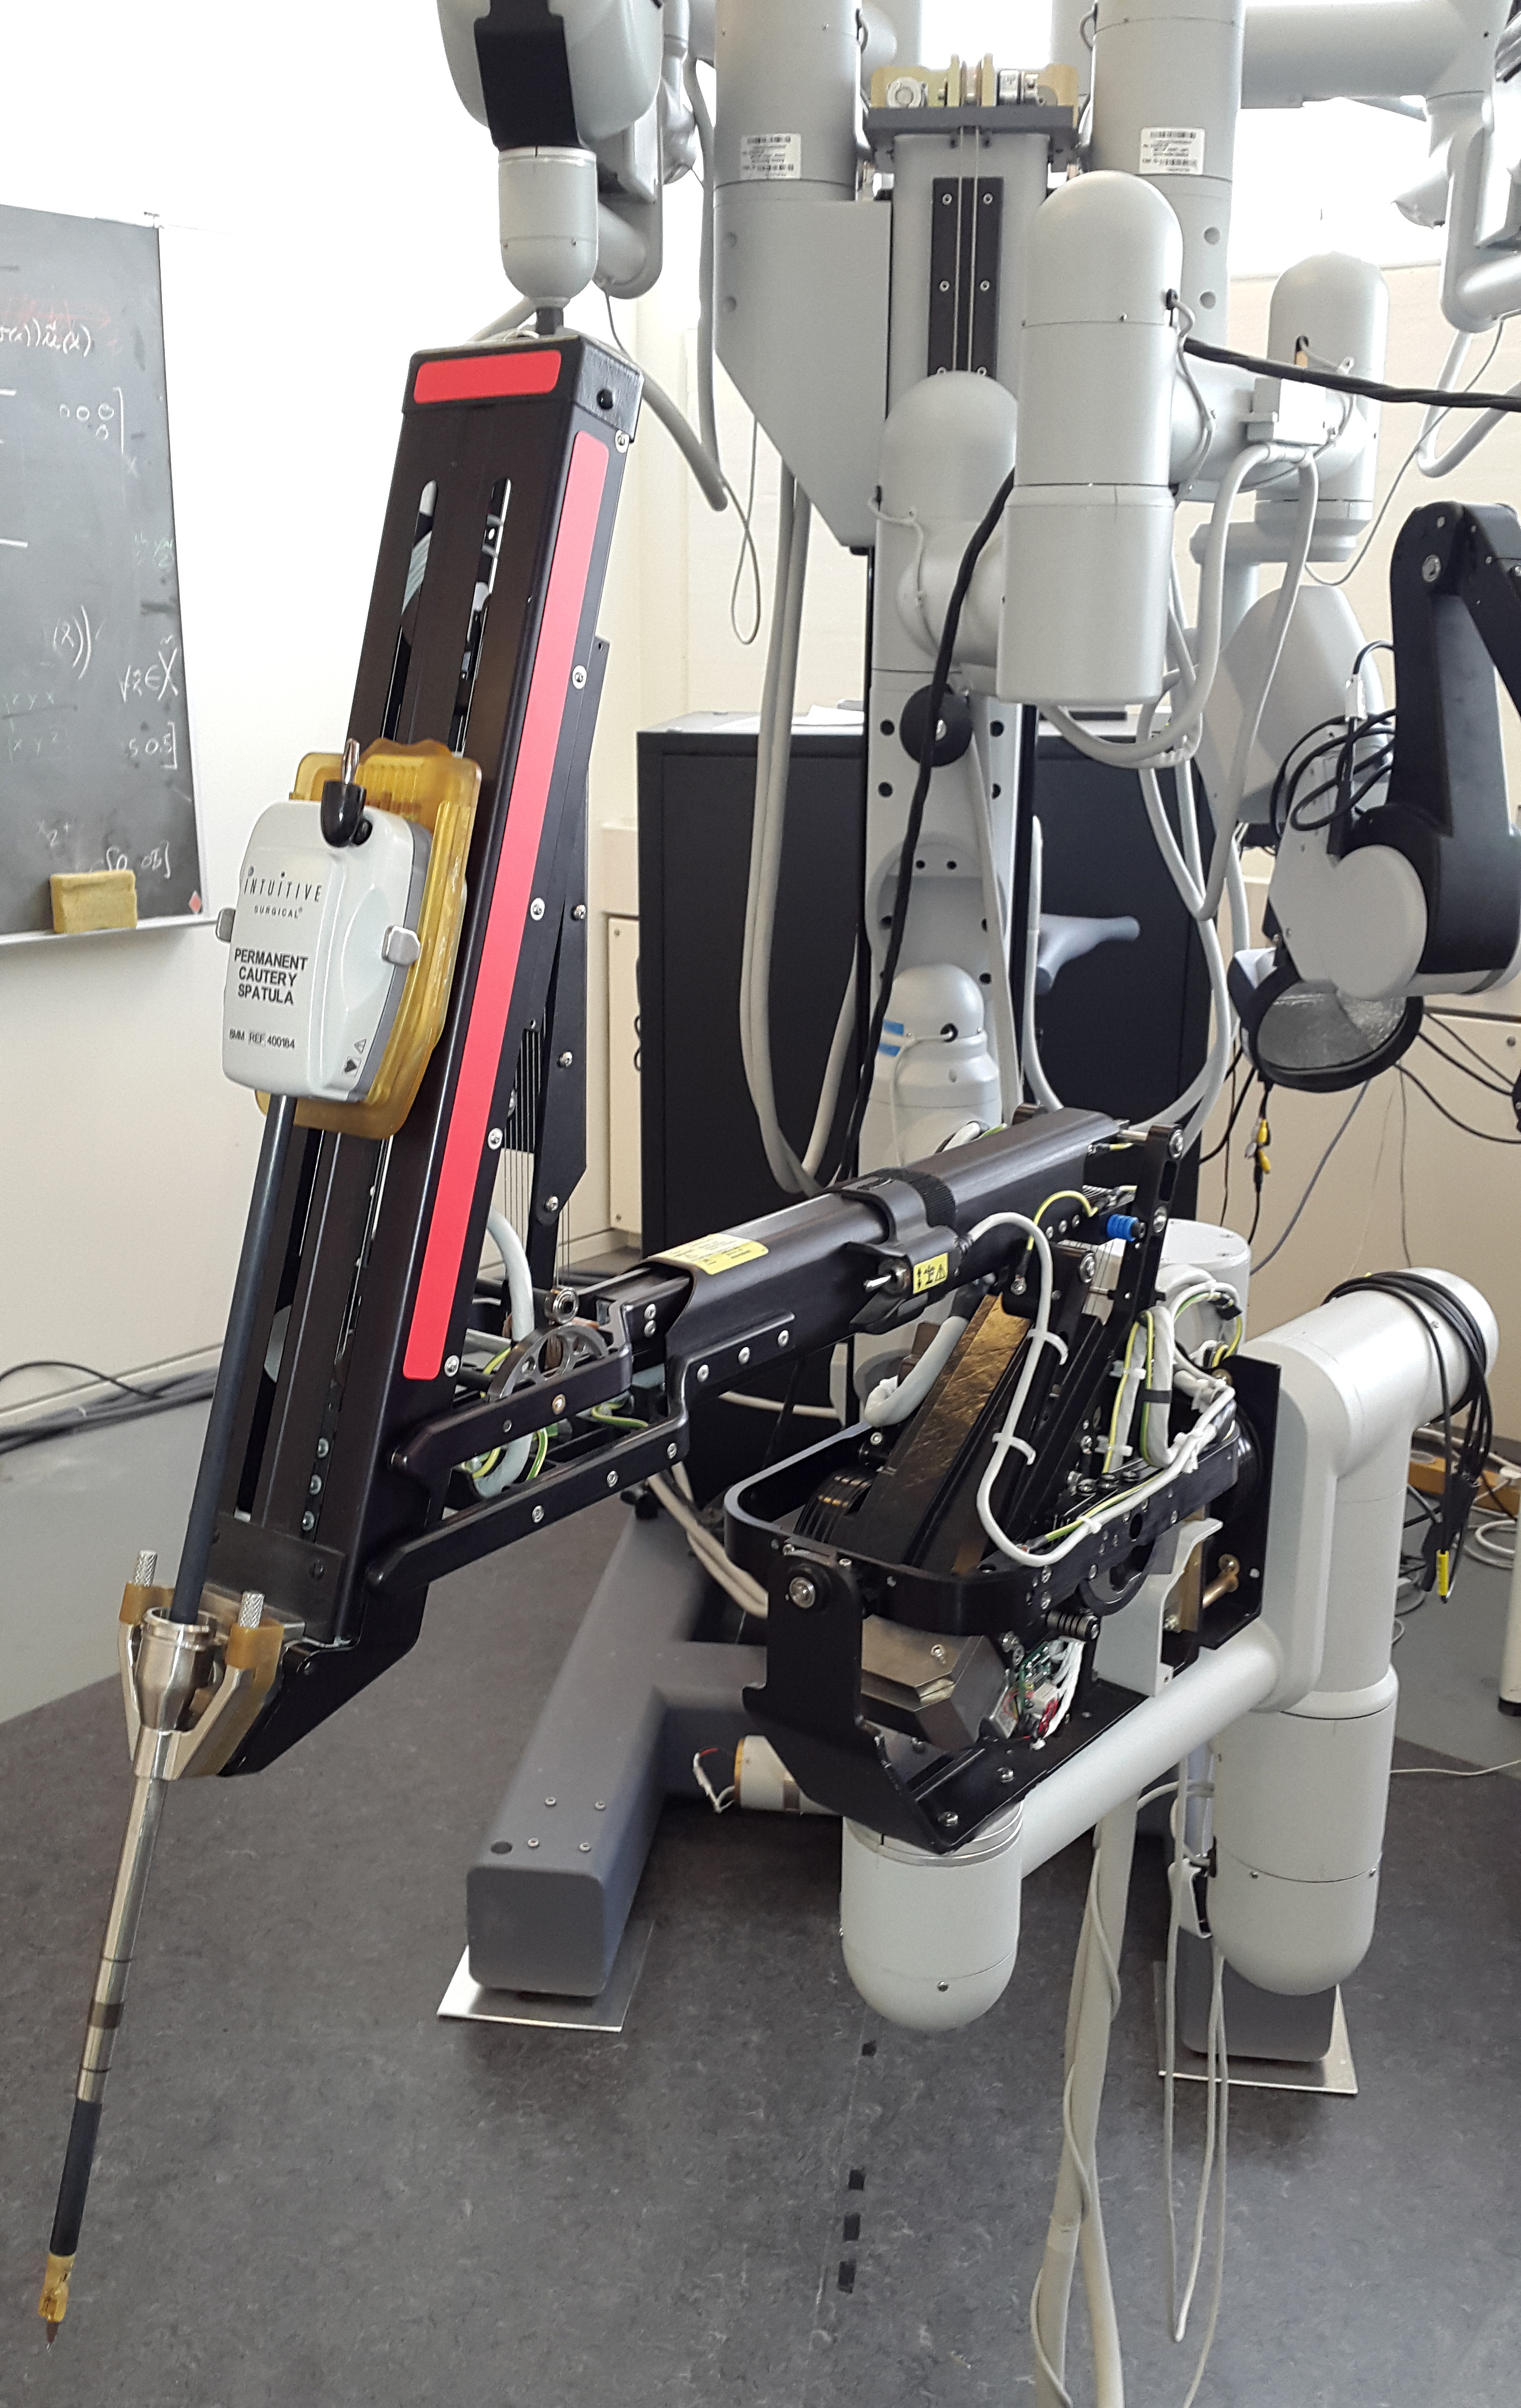
\includegraphics[width=1\textwidth]{20150517_120236.jpg}
%	\end{figure}
%\end{minipage}
%\vspace{1cm}
\begin{minipage}{0.35\textwidth}
	\vspace{-60mm}
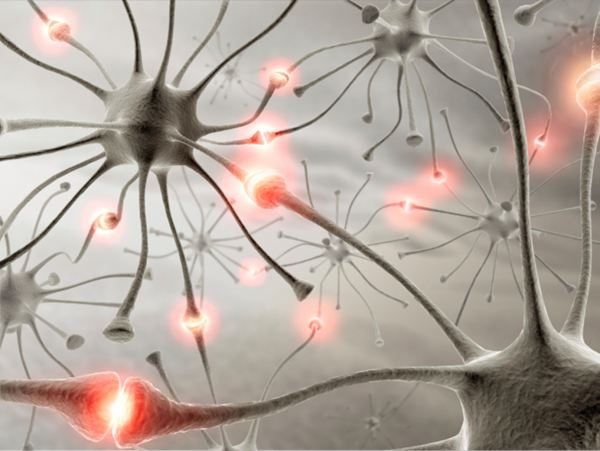
\includegraphics[width=\textwidth]{nerves.jpg}
\vspace{2mm}
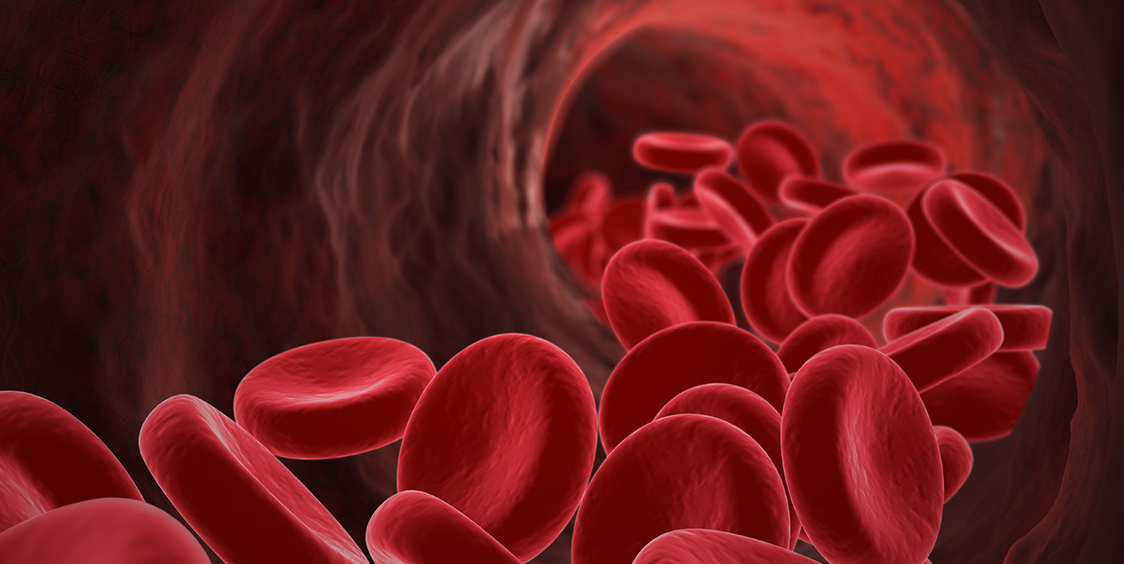
\includegraphics[width=\textwidth]{Blood-Clots-in-Vein.jpg}
\vspace{2mm}
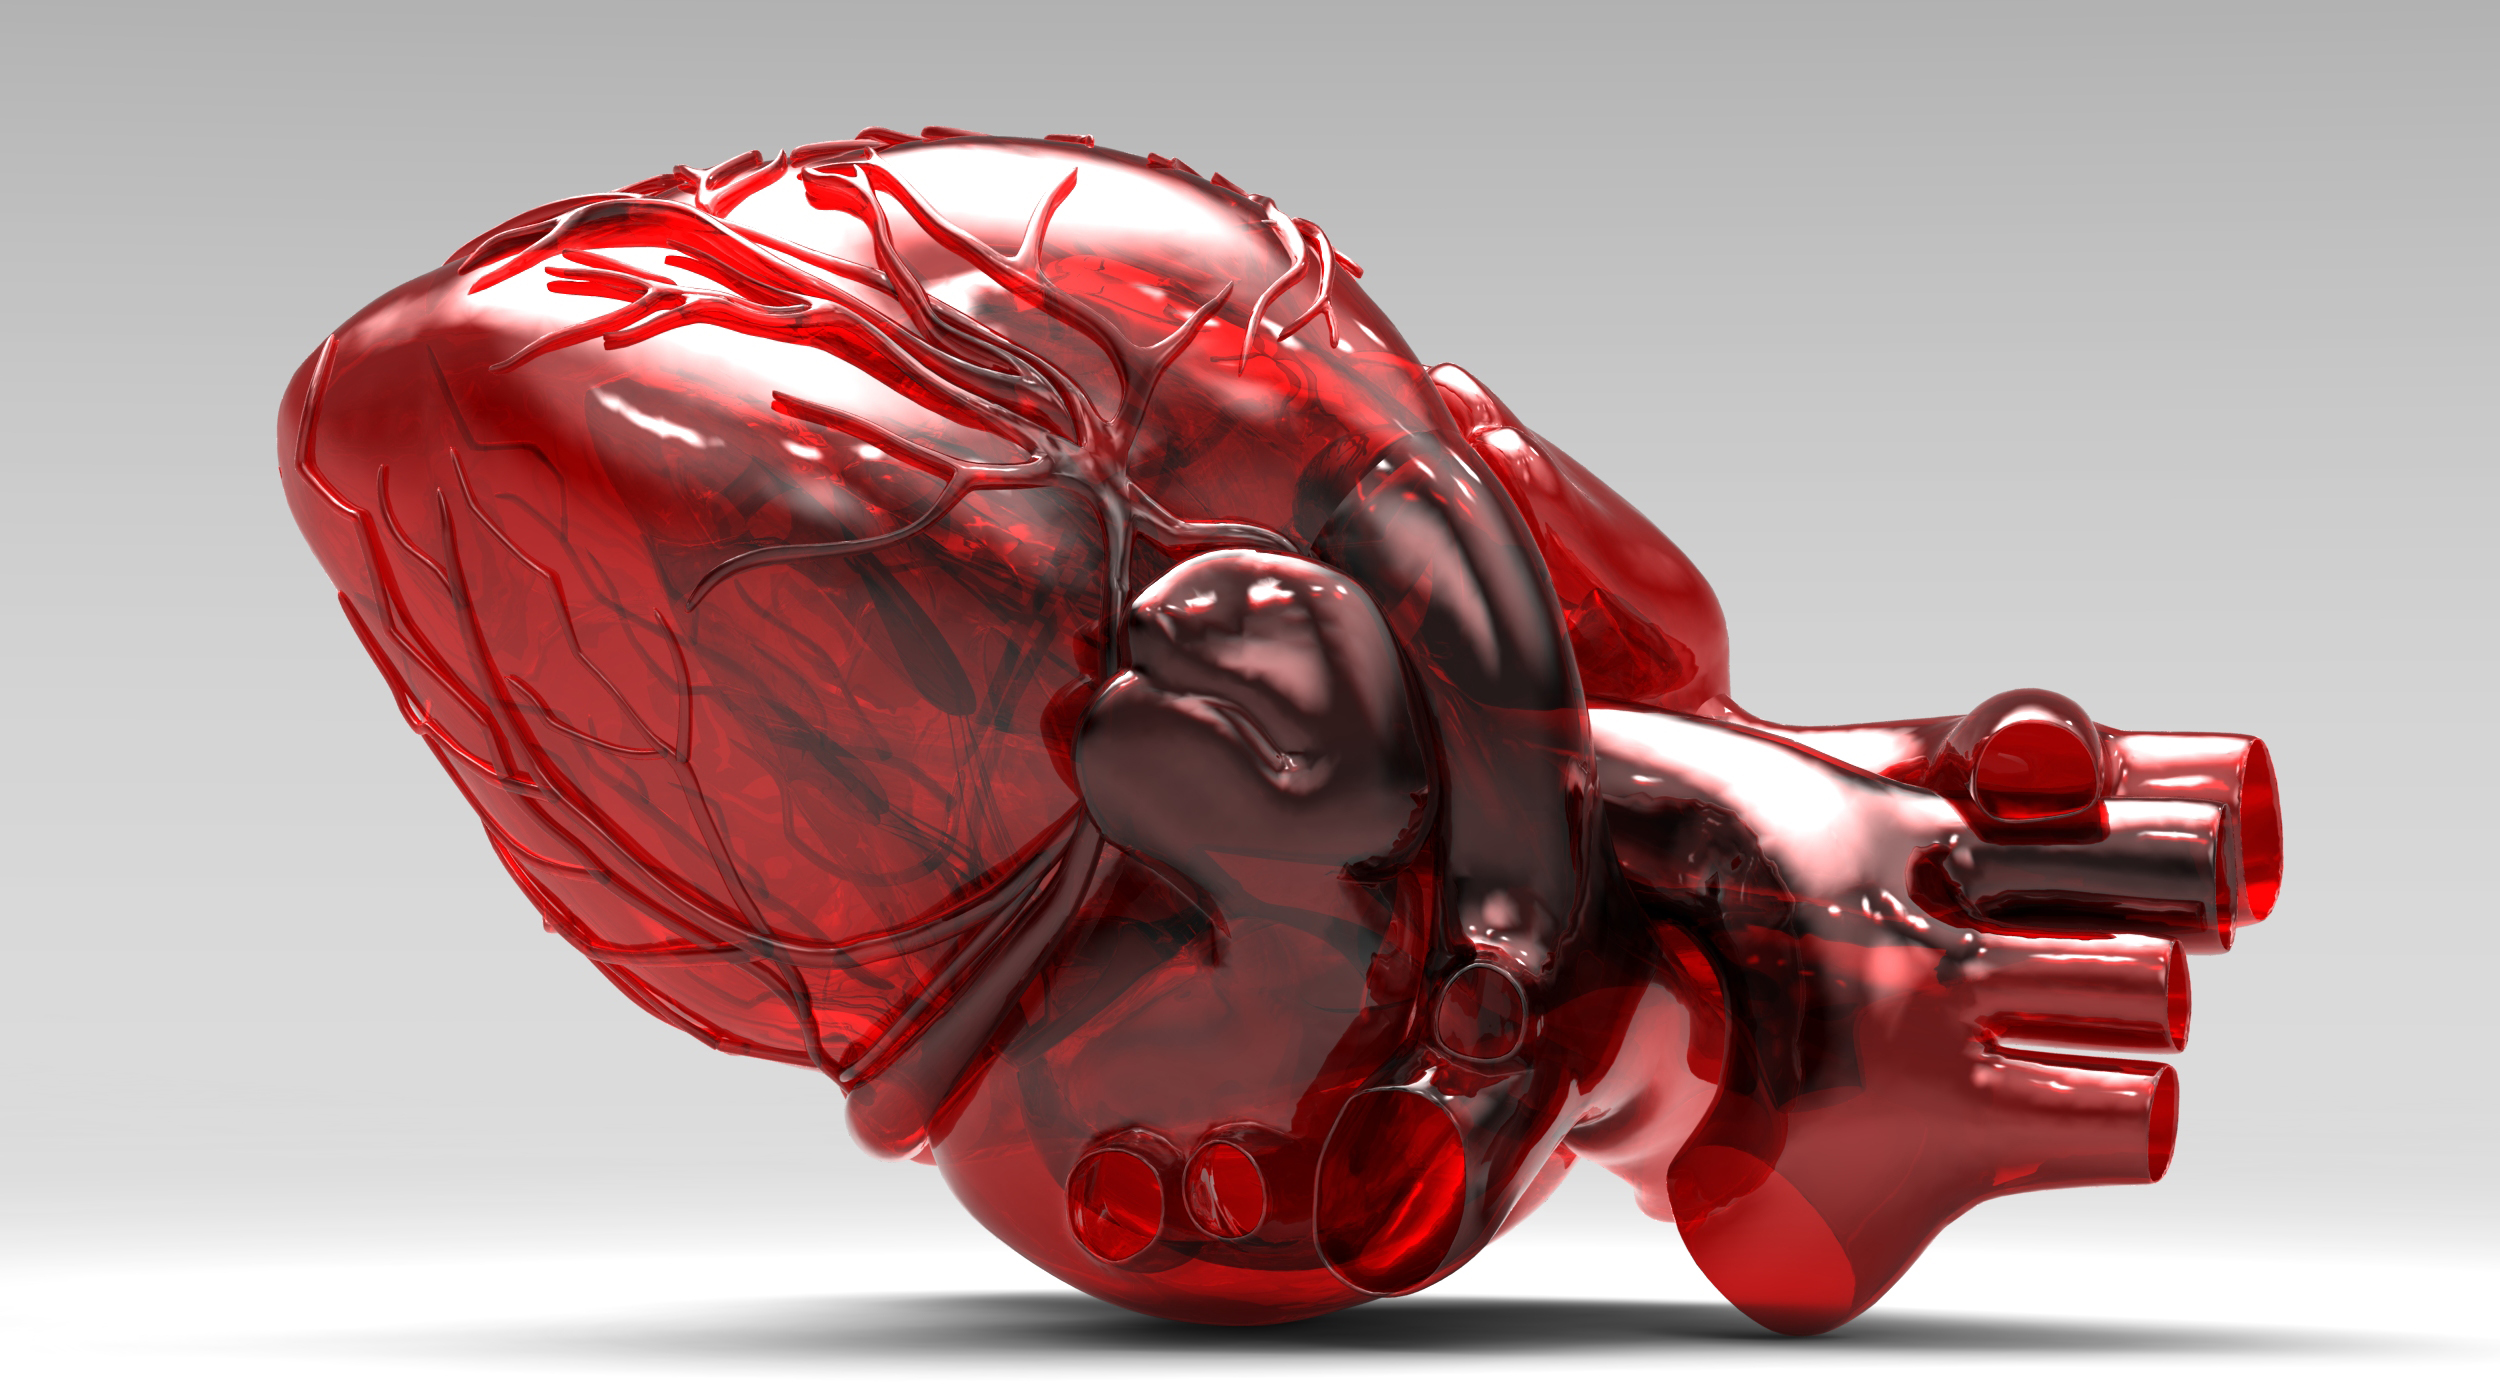
\includegraphics[width=\textwidth]{COLOURBOX6514659.jpg}
\end{minipage}

\end{frame}

\section{Barrierecertifikater}
\begin{frame}{Barrierecertifikater}{Formelt bevis for garanteret sikkerhed}
\vspace{2mm}
\begin{block}{Definition af sikkerhed}
	\begin{itemize}
		\item Systemets tilstande er i $\mathcal{X}$
		\item Usikre tilstande er i $\mathcal{X}_u\subset\mathcal{X}$ og sikre tilstande i $\mathcal{X}_0\subseteq\mathcal{X}\setminus\mathcal{X}_u$
		\item Nulniveaukurven af $B(\textbf{x})$ danner  barriere mellem $\mathcal{X}_0$ og $\mathcal{X}_u$
	\end{itemize}
\end{block}
\begin{minipage}[b]{0.4\linewidth}
	\vspace{2mm}
	\begin{block}{Barrierecertifikat}
		\vspace{-5mm}
	\begin{align*}
	B(\mathbf{x})&\leq 0 \quad \forall\,\,\,\mathbf{x}\in\mathcal{X}_0\\
	B(\mathbf{x})&> 0 \quad \forall\,\,\,\mathbf{x}\in\mathcal{X}_u\\
	L_{f_{cl}}B(\mathbf{x})&\leq 0 \quad \forall\,\,\,\mathbf{x}\in\mathcal{X}
	\end{align*}
	\vspace{-5mm}
	\begin{itemize}
		\item for systemet $\dot{\mathbf{x}}=f_{cl}$
	\end{itemize}
\end{block}
\end{minipage}
\hspace{2mm}
\begin{minipage}[b]{0.55\linewidth}
\begin{figure}[h]
	\centering
	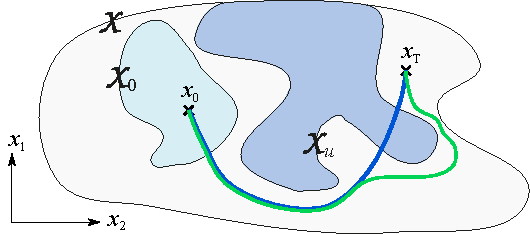
\includegraphics[width=\textwidth]{safety.pdf}
\end{figure}
\end{minipage}
\end{frame}

\section{Kontroldesign}
\begin{frame}{Kontrolbarrierefunktioner (CBF)}{Konstruktion af CBF til design af sikkerhedsregulator}
	\vspace{3mm}
\begin{minipage}[b]{0.5\linewidth}
	\begin{block}{Definition af CBF}
		\vspace{-5mm}
		\begin{align*}
		\mathbf{x}\in\mathcal{X}_u \,\,\, \Rightarrow\,\,\, B(\mathbf{x})&>0\\
		L_gB(\mathbf{x})=0 \,\,\,\Rightarrow\,\,\, L_fB(\mathbf{x})&<0\\
		\{\mathbf{x}\in\mathcal{X}\,\,|\,\,B(\mathbf{x})\leq 0 \} &\neq \emptyset
		\end{align*}
	\end{block}
\end{minipage}
\hspace{4mm}
\begin{minipage}[b]{0.35\linewidth}
	\begin{block}{Barrierecertifikat}
		\vspace{-5mm}
		\begin{align*}
		B(\mathbf{x})&\leq 0 \quad \forall\,\,\,\mathbf{x}\in\mathcal{X}_0\\
		B(\mathbf{x})&> 0 \quad \forall\,\,\,\mathbf{x}\in\mathcal{X}_u\\
		L_{f_{cl}}B(\mathbf{x})&\leq 0 \quad \forall\,\,\,\mathbf{x}\in\mathcal{X}
		\end{align*}
	\end{block}
\end{minipage}
\vspace{-2mm}
\begin{itemize}
	\item for systemet $\dot{\mathbf{x}}=f_{cl}(\mathbf{x})=f(\mathbf{x})+g(\mathbf{x})u$
\end{itemize}
\vspace{4mm}
\begin{block}{Kombination af to regulatorer}
	\begin{itemize}
		\item Lineær positionskontrol $\tilde{u}(\mathbf{x})$ indenfor det sikre område $\mathcal{X}_0$
%		\begin{equation*}
%		\tilde{u}(\mathbf{x})=\bar{\mathbf{N}}\mathbf{x}_\text{ref}-\mathbf{K}\mathbf{x}
%		\end{equation*}
		\item Sikkerhedsregulator $k_0(\mathbf{x})$ designet vha. CBF % så krav til sikkerhed bliver opfyldt
%		\begin{equation*}
%		k_0(\mathbf{x})=-\frac{L_fB(\mathbf{x})+\sqrt{L_fB(\mathbf{x})^2+\kappa^2L_gB(\mathbf{x})L_gB(\mathbf{x})^T}}{L_gB(\mathbf{x})L_gB(\mathbf{x})^T}L_gB(\mathbf{x})^T
%		\end{equation*}
		\item Gradvis overgang til sikkerhedsregulator nær $\mathcal{X}_u$
		\vspace{-1mm}
		\begin{equation*}
		u(\mathbf{x},\tilde{u})=\sigma(\mathbf{x})k_0(\mathbf{x})+(1-\sigma(\mathbf{x}))\tilde{u}(\mathbf{x})
		\end{equation*}
%		\vspace{-2mm}
	\end{itemize}
\end{block}


%\begin{figure}[h]
%	\centering
%	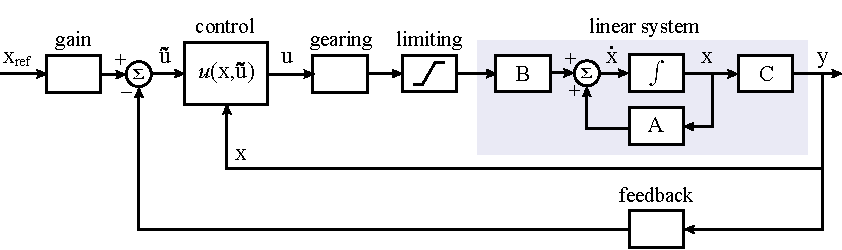
\includegraphics[width=0.9\textwidth]{control_system.pdf}
%\end{figure}
	\vspace{5mm}
\end{frame}